%!TeX root=../thesis.tex
%("dica" para o editor de texto: este arquivo é parte de um documento maior)
% para saber mais: https://tex.stackexchange.com/q/78101/183146

\chapter{The SPIRA ML-Enabled System}
\label{chap:the_spira_system}
%%%%%%%%%%%%%%%%%%%%%%%%%%%%%%%%%%%%%%%%%%%%%%%%%%%%%%%%%%%%%%%%%%%%%%%%%%%%%%%%

In 2020, amidst the COVID-19 pandemic, a multidisciplinary team of
researchers from the University of São Paulo (USP) created SPIRA:
a project to detect respiratory insufficiency via voice, using
Machine Learning (ML)~\parencite{Finger2021DetectingProject}.
This chapter describes the architecture of the SPIRA ML-enabled
system, as illustrated by \cref{fig:spira_architecture}.
\Crefrange{sec:spira_data_collection}{sec:spira_continuous_delivery}
showcase the six subsystems of the reference architecture introduced
in \cref{chap:ml_enabled_systems}. 
% components are grouped according to the subsystems
% On a note, the \cref{sec:spira_serving} subsystem also includes components
% of the client application, since the client was also developed in the
% context of the project.

In the early days of the COVID-19 pandemic, there were no clinical exams
to diagnose the illness. Patients would show up in hospitals with a low
level of oxygen in the blood, but they were not feeling any effects --
becoming ``breathless'' -- until their lungs were severely compromised.
SPIRA was created with the idea of using \emph{speech recognition}%
~\parencite{RussellS2021Artificial4th} to find early signs of
respiratory insufficiency, thus helping physicians to identify
which patients needed urgent treatment.

Currently, the scope of the SPIRA project has evolved. Its proposal
is to detect respiratory insufficiency of any origin, while ideally
identifying which illness may originate it. Some examples of other
sickness that cause respiratory insufficiency include smoking
side effects, flu, severe asthma, and heart condition%
~\parencite{Finger2021DetectingProject}.

%----------------------------------------------------------------------------%
\begin{figure}[p]
  \centering
  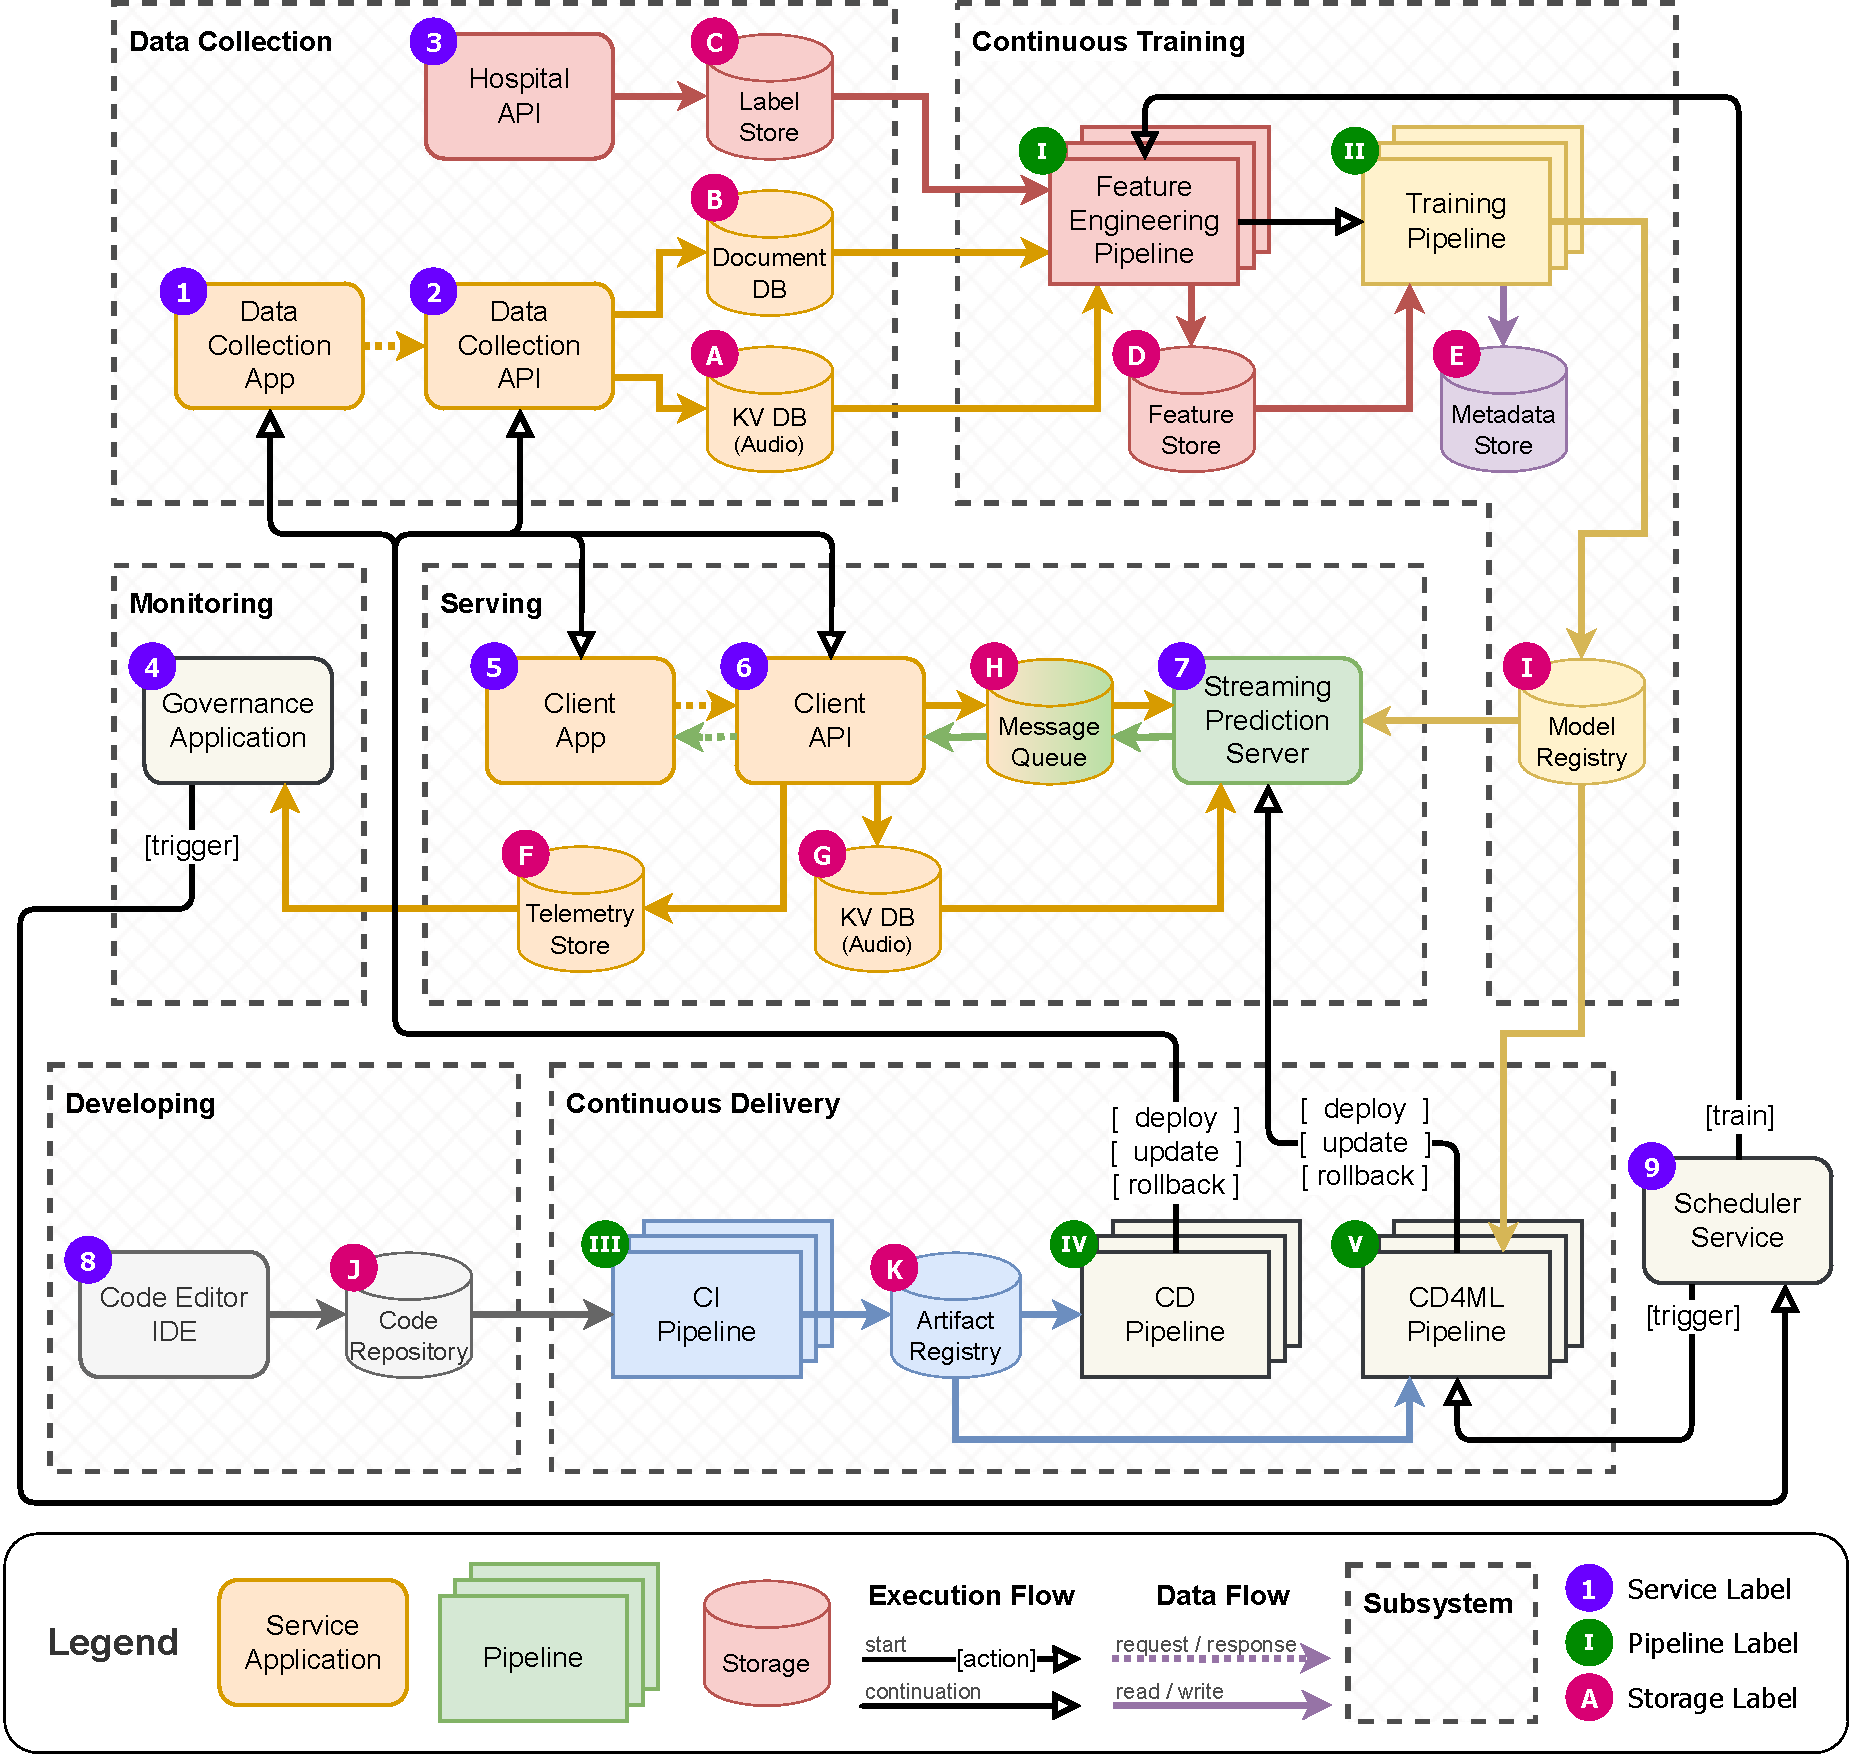
\includegraphics[width=\linewidth]{figures/SPIRA.pdf}
  \caption[%
    Architecture of the SPIRA ML-enabled system%
  ]{%
    \emph{Architecture of the SPIRA ML-enabled system.}
    This architecture follows the same notation presented in
    \cref{fig:reference_architecture}.
    Rectangles represent \textbf{applications} or \textbf{services},
      which execute continuously.
    Stacked rectangles represent \textbf{pipelines},
      which execute a task on demand.
    Lastly, cylinders represent \textbf{data storage},
      which may be databases of any type.
    Components are connected by arrows.
    Black arrows with a hollow tip illustrate the \textbf{execution flow}.
      They start and end in a component.
      Labeled arrows represent the trigger that starts a workflow,
      whereas unlabeled arrows represent the continuation of an
      existing workflow.
    Colored arrows with a filled tip illustrate the \textbf{data flow}.
    They appear in two types:
      solid arrows going to and from a data storage represent
      write and read operations, respectively;
      dotted arrows represent a sync or async request-response
      communication between components.
    Components are colored according to the data they produce:
      \mbox{\LegendColoredComponent{orange}{raw data}},
      \mbox{\LegendColoredComponent{red}{ML-specific data}},
      \mbox{\LegendColoredComponent{gray}{source code}},
      \mbox{\LegendColoredComponent{blue}{executable artifacts}},
      \mbox{\LegendColoredComponent{yellow}{ML models}},
      \mbox{\LegendColoredComponent{purple}{ML training metadata}},
      \mbox{\LegendColoredComponent{green}{ML model predictions}}, and
      \mbox{\LegendColoredComponent{pink}{ML model metrics}}.
      Remaining \LegendBWComponent{standalone components} orchestrate
      the execution of others.
    Components are also grouped into \textbf{subsystems}.
    \LegendColoredLabel{violet}{Numbers},
    \LegendColoredLabel{moss}{roman numerals} and
    \LegendColoredLabel{magenta}{letters}
    are used as labels throughout \cref{chap:the_spira_system}.
  }
  \label{fig:spira_architecture}
\end{figure}
%----------------------------------------------------------------------------%

To create a tool that could assist physicians, the SPIRA team proposed
to develop an ML-enabled system. \Cref{fig:spira_architecture}
presents its system architecture, designed in the early days of this PhD
research~\parencite{Ferreira2022SPIRA:Detection}.
This section discusses how this architecture matches the reference
architecture in \cref{chap:ml_enabled_systems}.
Moreover, it explains how its components have been developed since 2021
through different projects supervised in the context of this research.
In 2022, the experience report \emph{\citetitle{Ferreira2022SPIRA:Detection}}%
~\parencite{Ferreira2022SPIRA:Detection}, was published in the 2nd Workshop
of Intelligent Software Engineering (ISE) at the Brazilian Conference on
Software: Practice and Theory (CBSoft).

A proof of concept of the SPIRA Machine Learning (ML) model was
published in the journal paper \emph{\citetitle{Casanova2021DeepSpeech}}%
~\parencite{Casanova2021DeepSpeech}. To detect respiratory insufficiency
via voice, \citeauthor{Casanova2021DeepSpeech} proposed using
a Convolutional Neural Network (CNN) with multiple hidden layers%
~\parencite{IanGoodfellow2016DeepLearning,RussellS2021Artificial4th},
which could process audio signals recorded in a protocol.
Once they showed the problem could be solved, the next step
was to design an ML-enabled system that could support the proposed
model lifecycle. This way, the SPIRA team would have the means to
incrementally develop and test improvements to their solution.

% The next sections describe the components of the SPIRA system,
% as illustrated by \cref{fig:spira_architecture}. They are grouped
% according to the subsystems presented at \cref{sec:reference_architecture}. 
% On a note, the \cref{sec:spira_serving} subsystem also includes components
% of the client application, since the client was also developed in the
% context of the project.

  \section{Data Collection.}\label{sec:spira_data_collection}
  %%%%%%%%%%%%%%%%%%%%%%%%%%%%%%%%%%%%%%%%%%%%%%%%%%%%%%%%%%%%%%%%%%%%%%%%%%%%
  Creating an ML model that can detect respiratory insufficiency
  via voice is a supervised machine learning classification problem%
  ~\parencite{Casanova2021DeepSpeech}. As such, as explained in
  \cref{sec:ref_data_acquisition}, it requires \emph{labeled data}.
  For the proof of concept, \citeauthor{Casanova2021DeepSpeech}
  used samples obtained in an open survey form shared on the web.
  In the early days of the pandemic, this idea worked well,
  since many people were getting infected (unbeknownst to them).
  Therefore, the odds of finding positive and negative examples
  in the population were high.
  
  When the COVID-19 pandemic started becoming under control, the only
  way to reliably find people with respiratory insufficiency were in the
  hospitals. For that reason, in 2022, the SPIRA team started the development
  of a \LegendService{1}{data collection app}, which could be used by volunteer
  data collectors (working in hospitals) to gather voices.
  This Progressive Web App (PWA) would send the data to a
  \LegendPipeline{2}{data collection API}, which in turn would
  store audio in an \LegendDataStore{A}{audio key-value database}, and
  save patients' demographic data in a \LegendDataStore{B}{document database}.
  These components were developed in the supervision of a scientific
  initiation by the bachelor student Francisco Eugenio Wernke, who developed
  them as part of the course MAC0215 -- ``Undergraduate Research'' at IME-USP.
  %--------------------------------------------------------------------------%
  \begin{supervision}
    \label{sup:ic_francisco}
    \noindent\textbf{%
      Developing a PWA for Collecting Voice for the SPIRA Project.
    }
  
    \noindent%
    \emph{%
      Francisco Eugenio Wernke,
      Renato Cordeiro Ferreira,
      Alfredo Goldman.
    }
  \noindent%
    Scientific Initiation (Bachelor of Computer Science).
  
    \noindent%
    Institute of Mathematics and Statistics, University of São Paulo, 2021.
  \end{supervision}
  %--------------------------------------------------------------------------%
  
  After each collect, data collectors registered an identifier
  (RGH, \EnToBr{Registro Geral Hospitalar}) for each participant.
  This identifier could later be cross-referenced with data shared by each
  partner hospitals via \LegendService{3}{Hospital APIs}. This way, the
  researchers could create a \LegendDataStore{C}{label store} that
  would provide a \emph{ground truth} for the system.
  
  \section{Continuous Training.}\label{sec:spira_continuous_training}
  %%%%%%%%%%%%%%%%%%%%%%%%%%%%%%%%%%%%%%%%%%%%%%%%%%%%%%%%%%%%%%%%%%%%%%%%%%%%
  The next step to productionize SPIRA was to enable continuous training.
  The proof-of-concept code shared by \citeauthor{Casanova2021DeepSpeech}
  could be transformed into two new components:
    a \LegendPipeline{I}{feature engineering pipeline},
    to handle all data processing steps to make audio signals consumable
    by the training algorithm; and
    a \LegendPipeline{II}{training pipeline}, to train and validate the CNN
    proposed in the proof of concept~\parencite{Casanova2021DeepSpeech}.
  
  As explained in \cref{sec:ref_continuous_training}, the creation of these
  two pipelines is an opportunity to introduce standard machine learning
  design patterns~\parencite{Lakshmanan2020MachineMLOps}, such as
    a \LegendDataStore{D}{feature store},
    a \LegendDataStore{E}{metadata store}, and
    a \LegendDataStore{I}{model registry}.
  For the purposes of the project, the suggestion was to use
  \href{https://mlflow.org}{MLFlow} to make the two latter roles.
  On the other hand, for the features, the proposal was to use a
  simple key-value database like \href{https://min.io}{MinIO},
  since a full-featured tool like \href{https://feast.dev}{Feast}
  would be overkill for managing features for a single ML-enabled system.
  
  The implementation of the \nameref{sec:spira_continuous_training}
  subsystem was split into two parts. In 2023, the bachelor student
  Daniel Lawand studied the codebase published by
  \citeauthor{Casanova2021DeepSpeech}~\parencite{Casanova2021DeepSpeech},
  to propose a redesign to its structure. The goal was to evaluate how
  to clean the experimental code, focusing on maintainability.
  This project was supervised as part of Daniel's capstone project.
  In late 2023, it was partially developed in an exchange
  to the Jheronimus Academy of Data Science (JADS) in the Netherlands.
  %--------------------------------------------------------------------------%
  \begin{supervision}
    \label{sup:tcc_daniel}
    \noindent\textbf{%
      Enabling MLOps in the SPIRA training pipeline.
    }
  
    \noindent%
    \emph{%
      Daniel Lawand,
      Renato Cordeiro Ferreira,
      Alfredo Goldman.
    }
  
    \noindent%
    Capstone Project (Bachelor of Computer Science).
  
    \noindent%
    Institute of Mathematics and Statistics, University of São Paulo, 2023.
  \end{supervision}
  %--------------------------------------------------------------------------%
  
  In 2024, the bachelor students Lucas Quaresma and Roberto Bolgheroni
  are continuing this task. Their goal is to implement the design proposal
  made by Daniel Lawand. This project was supervised as part of Lucas's
  and Roberto's group capstone projects. In late 2024, it will be concluded
  in an upcoming exchange of the students to the Jheronimus Academy of
  Data Science (JADS) in the Netherlands.
  %--------------------------------------------------------------------------%
  \begin{supervision}
    \label{sup:tcc_lucas_roberto}
    \noindent\textbf{%
      Productionizing the SPIRA Continuous Training Pipeline.
    }
  
    \noindent%
    \emph{%
      Lucas Quaresma,
      Roberto Bolgheroni,
      Renato Cordeiro Ferreira,
      Alfredo Goldman.
    }
  
    \noindent%
    Capstone Project (Bachelor of Computer Science).
  
    \noindent%
    Institute of Mathematics and Statistics, University of São Paulo, 2024.
  \end{supervision}
  %--------------------------------------------------------------------------%
  
  \section{Serving}\label{sec:spira_serving}
  %%%%%%%%%%%%%%%%%%%%%%%%%%%%%%%%%%%%%%%%%%%%%%%%%%%%%%%%%%%%%%%%%%%%%%%%%%%%
  
  Given SPIRA was meant to be used in hospitals, the client application
  needs to be prepared for this environment. Among the challenges,
  hospitals can have poor internet reception, considering the way
  their building are built (with many corridors and walls).
  As a consequence, the \LegendService{5}{client app} needs to store
  all data collected locally \emph{before} sending them to the cloud,
  thus preventing problems with an unreliable network. This implies
  the \LegendService{6}{client API} should also make a checksum of
  any data received to ensure everything no data was corrupted before
  storing it in its \LegendDataStore{G}{audio key-value database}.
  Moreover, data will likely arrive in \emph{bursts}, i.e., multiple
  audios will be sent together by the \LegendService{5}{client app}
  when the data collector gets internet access.
  
  To handle an arbitrarily large, unforeseeable, on-demand number
  of predictions, SPIRA should rely on a \LegendService{7}{streaming
  prediction service}. It will queue all prediction requests in a
  \LegendDataStore{H}{message queue}, then return the predictions
  results through it. This solution also makes it easier to manage
  the execution of the server.
  The model proposed by \citeauthor{Casanova2021DeepSpeech} -- a CNN with
  multiple layers -- is a model that requires accelerator hardware (GPUs)
  to run efficiently~\parencite{IanGoodfellow2016DeepLearning}.
  The \LegendService{7}{streaming prediction service} can be run
  in a specialized machine, whereas other components may be
  deployed in cheaper hardware.
  
  The implementation of the \nameref{sec:spira_serving} subsystem was also
  split in two parts. In 2022, the bachelor student Vitor Tamae developed
  all the components in the subsystem.
  %--------------------------------------------------------------------------%
  \begin{supervision}
    \label{sup:tcc_tamae}
    \noindent\textbf{%
      Building an Intelligent System to Detect Respiratory Insufficiency.
    }
  
    \noindent%
    \emph{%
      Vitor Daisuke Tamae,
      Renato Cordeiro Ferreira,
      Marcelo Finger,
      Alfredo Goldman.
    }
  
    \noindent%
    Capstone Project (Bachelor of Computer Science).
  
    \noindent%
    Institute of Mathematics and Statistics, University of São Paulo, 2022.
  \end{supervision}
  %--------------------------------------------------------------------------%
  
  In 2023, the bachelor student Vitor
  Guidi continued this effort by investigating how to deploy all this
  infrastructure in a \href{https://kubernetes.io/}{Kubernetes}-managed
  cluster of machines. Both projects were supervised as part of the
  students' capstone projects.
  %--------------------------------------------------------------------------%
  \begin{supervision}
    \label{sup:tcc_guidi}
    \noindent\textbf{%
      Cloud-Native Machine Learning: \\
      Enabling High Availability to the SPIRA System with Kubernetes.
    }
  
    \noindent%
    \emph{%
      Vitor Guidi,
      Renato Cordeiro Ferreira,
      Alfredo Goldman.
    }
  
    \noindent%
    Capstone Project (Bachelor of Computer Science).
  
    \noindent%
    Institute of Mathematics and Statistics, University of São Paulo, 2023.
  \end{supervision}
  %--------------------------------------------------------------------------%
  
  \section{Monitoring.}\label{sec:spira_monitoring}
  %%%%%%%%%%%%%%%%%%%%%%%%%%%%%%%%%%%%%%%%%%%%%%%%%%%%%%%%%%%%%%%%%%%%%%%%%%%%
  Another desirable capability for the SPIRA system is AB-testing,
  so it may be possible to train and test multiple variants of the SPIRA
  CNN to improve its modelling. As part of his capstone project,
  while implementing the \nameref{sec:spira_serving} subsystem,
  the bachelor student Vitor Tamae made the \LegendService{6}{client API}
  to support calling multiple models at the same time. This capability is
  the inception of a \LegendService{4}{governance application}, which will
  allow the researchers to track the system usage stored in a
  \LegendDataStore{F}{telemetry store}.
  
  \section{Development.}
  \label{sec:spira_development_ci}
  %%%%%%%%%%%%%%%%%%%%%%%%%%%%%%%%%%%%%%%%%%%%%%%%%%%%%%%%%%%%%%%%%%%%%%%%%%%%
  The last step to support further experimentation with the SPIRA model
  is to provide the capability to quickly experiment with multiple systems.
  Currently, data scientists can access SPIRA source code in an open
  \LegendDataStore{J}{code repository} at GitHub%
  \footnote{https://github.com/spirabr}.
  Any changes may be made using standard development tools:
  \LegendService{8}{code editors} or \LegendService{8}{IDEs},
  according to the preference of the SPIRA team.
  
  \section{Continuous Delivery.}
  \label{sec:spira_continuous_delivery}
  %%%%%%%%%%%%%%%%%%%%%%%%%%%%%%%%%%%%%%%%%%%%%%%%%%%%%%%%%%%%%%%%%%%%%%%%%%%%
  Taking advantage of the use of \href{https://github.com}{GitHub},
  the bachelor students Lucas Quaresma and Roberto Bolgheroni are currently
  building the \nameref{sec:spira_continuous_delivery} components to make
  it easy to build, test, and deploy new versions of SPIRA.
  The \LegendService{III}{CI pipeline} is being built using GitHub actions,
  to generate \href{https://www.docker.com/}{Docker} containers of the
  various components that are part of SPIRA. These containers will be
  deployed in the GitHub Container Registry%
  \footnote{https://github.blog/2020-09-01-introducing-github-container-registry/},
  which will be the \LegendDataStore{K}{artifact store} for SPIRA.
  
  During 2024, as part of their capstone project, the students
  Lucas Quaresma and Roberto Bolgheroni will also develop the
  \LegendPipeline{IV}{CD} and \LegendPipeline{V}{CD4ML} pipelines.
  They will use the infrastructure configuration developed by Vitor Guidi
  in 2023 to create a process to deploy, update, and rollback all components
  in a \href{https://kubernetes.io/}{Kubernetes}-managed cluster.
